\documentclass[11pt,a4paper]{article}

% ==============================================================================
% PACKAGES & TYPOGRAPHY (XeLaTeX)
% ==============================================================================
\usepackage{fontspec}
\setmainfont{Times New Roman}
\setsansfont{Arial}
\setmonofont{Consolas}

\usepackage[top=2.2cm, bottom=2.2cm, left=2.3cm, right=2.3cm, headheight=28pt]{geometry}
\setlength{\emergencystretch}{2.5em}
\tolerance=800
\usepackage{graphicx}
\usepackage{xcolor}
\usepackage{colortbl}
\usepackage{booktabs}
\usepackage{tabularx}
\usepackage{longtable}
\usepackage{array}
\usepackage{multirow}
\usepackage{float}
\usepackage{enumitem}
\usepackage{titlesec}
\usepackage{fancyhdr}
\usepackage{lastpage}
\usepackage{amsmath}
\usepackage{amssymb}
\usepackage{tikz}
\usetikzlibrary{arrows.meta,positioning,shapes.geometric,calc,fit,backgrounds}

\usepackage[colorlinks=true,linkcolor=brandblue,urlcolor=brandblue,citecolor=brandblue]{hyperref}

% ==============================================================================
% CORPORATE COLOR PALETTE
% ==============================================================================
\definecolor{brandnavy}{HTML}{0F172A}
\definecolor{brandblue}{HTML}{1640CA}
\definecolor{accentteal}{HTML}{0E4D64}
\definecolor{accentorange}{HTML}{D95D1E}
\definecolor{accentred}{HTML}{991B1B}
\definecolor{accentgreen}{HTML}{166534}
\definecolor{lightslate}{HTML}{F1F5F9}
\definecolor{softblue}{HTML}{EFF6FF}
\definecolor{softamber}{HTML}{FFFBEB}
\definecolor{softred}{HTML}{FEF2F2}
\definecolor{softgreen}{HTML}{F0FDF4}
\definecolor{bordergray}{HTML}{CBD5E1}
\definecolor{mutedtext}{HTML}{475569}

% ==============================================================================
% CUSTOM COLUMN TYPES & SPACING
% ==============================================================================
\newcolumntype{L}[1]{>{\raggedright\arraybackslash}p{#1}}
\newcolumntype{C}[1]{>{\centering\arraybackslash}p{#1}}
\newcolumntype{R}[1]{>{\raggedleft\arraybackslash}p{#1}}
\newcolumntype{Y}{>{\raggedright\arraybackslash}X}

\setlength{\parindent}{0pt}
\setlength{\parskip}{6pt}
\renewcommand{\arraystretch}{1.28}

% ==============================================================================
% SECTION STYLING (Clean Corporate / Word-like Hierarchy)
% ==============================================================================
\renewcommand{\contentsname}{DAFTAR ISI}
\renewcommand{\figurename}{Gambar}
\renewcommand{\tablename}{Tabel}

\titleformat{\section}
  {\sffamily\large\bfseries\color{brandnavy}}
  {\thesection.}{0.6em}{}
  [\vspace{-0.4em}{\color{brandblue}\rule{\textwidth}{1.2pt}}]

\titleformat{\subsection}
  {\sffamily\normalsize\bfseries\color{accentteal}}
  {\thesubsection}{0.6em}{}

\titleformat{\subsubsection}
  {\sffamily\small\bfseries\color{brandnavy}}
  {\thesubsubsection}{0.6em}{}

\titlespacing*{\section}{0pt}{14pt}{6pt}
\titlespacing*{\subsection}{0pt}{10pt}{4pt}
\titlespacing*{\subsubsection}{0pt}{8pt}{2pt}

% ==============================================================================
% HEADER & FOOTER CONFIGURATION
% ==============================================================================
\pagestyle{fancy}
\fancyhf{}
\fancyhead[L]{\sffamily\scriptsize\color{mutedtext}PT SCHRYZON DIGITAL NUSANTARA | 3D\={e}x Commercial Platform}
\fancyhead[R]{\sffamily\scriptsize\color{mutedtext}Dokumen: \texttt{SDN-3DEX-PC-001} (v1.0)}
\fancyfoot[L]{\sffamily\scriptsize\color{mutedtext}\textit{Rahasia Perusahaan | Kepemilikan Komersial Klien (Krea3D Corp)}}
\fancyfoot[R]{\sffamily\scriptsize\color{mutedtext}Halaman \thepage\ dari \pageref{LastPage}}
\renewcommand{\headrulewidth}{0.5pt}
\renewcommand{\footrulewidth}{0.5pt}

% ==============================================================================
% VECTOR LOGO MACRO (Exact Isometric Hexagon from apps/frontend/public/3Dex.svg)
% ==============================================================================
\newcommand{\threedexlogo}[1][0.032pt]{%
\begin{tikzpicture}[x=#1, y=-#1, baseline=(current bounding box.center)]
  % Dark hexagon backdrop matching og-image.png badge
  \fill[brandnavy]
    (720, 29.32) -- (1418.5, 456.32) -- (1418.5, 1297.32) --
    (720, 1721.32) -- (25, 1297.32) -- (25, 456.32) -- cycle;
  % Blue facets (#1640CA)
  \fill[brandblue] (370, 278.32) -- (714, 62.32) -- (1020, 241.82) -- (370, 584.32) -- cycle;
  \fill[brandblue] (777, 431.82) -- (1068.5, 270.32) -- (1393, 472.82) -- (1393, 761.32) -- cycle;
  \fill[brandblue] (1135.5, 673.82) -- (1393, 817.82) -- (1393, 1283.32) -- (1135, 1440.32) -- cycle;
  \fill[brandblue] (1085, 1469.82) -- (1085, 1157.82) -- (447.5, 1525.32) -- (720.5, 1691.82) -- cycle;
  \fill[brandblue] (768, 866.82) -- (1082.5, 674.82) -- (1082.5, 1067.32) -- cycle;
  % White isometric wireframe strokes
  \draw[white, line width=1.45pt, line join=round, line cap=round]
    (1110, 1484.59) -- (720, 1721.32) -- (398, 1524.88)
    (1110, 1484.59) -- (1110, 1114.32)
    (1110, 1484.59) -- (1418.5, 1297.32) -- (1418.5, 802.32)
    (398, 1524.88) -- (720, 1341.32)
    (398, 1524.88) -- (25, 1297.32) -- (25, 924.32)
    (720, 1341.32) -- (1110, 1114.32)
    (720, 1341.32) -- (340.5, 1114.32)
    (1110, 1114.32) -- (1110, 629.32)
    (1110, 1114.32) -- (720, 866.82)
    (1110, 629.32) -- (1418.5, 802.32)
    (1110, 629.32) -- (720, 432.82)
    (1110, 629.32) -- (720, 866.82)
    (1418.5, 802.32) -- (1418.5, 456.32) -- (1069.25, 242.82)
    (720, 432.82) -- (1069.25, 242.82)
    (720, 432.82) -- (340.5, 629.32)
    (1069.25, 242.82) -- (720, 29.32) -- (340.5, 262.48)
    (340.5, 629.32) -- (340.5, 262.48)
    (340.5, 629.32) -- (720, 866.82)
    (340.5, 629.32) -- (340.5, 1114.32)
    (340.5, 262.48) -- (25, 456.32) -- (25, 924.32)
    (720, 866.82) -- (340.5, 1114.32)
    (340.5, 1114.32) -- (25, 924.32);
\end{tikzpicture}%
}

% Status pill helper
\newcommand{\badge}[2]{%
  \tikz[baseline=(char.base)]{\node[fill=#1, text=white, rounded corners=2pt, inner xsep=5pt, inner ysep=2pt, font=\sffamily\scriptsize\bfseries] (char) {#2};}%
}

% ==============================================================================
% DOCUMENT START
% ==============================================================================
\begin{document}

% ------------------------------------------------------------------------------
% PART I: SURAT PENGANTAR & PERMOHONAN PENGESAHAN PROJECT CHARTER (HALAMAN 1-2)
% ------------------------------------------------------------------------------
\pagestyle{empty}

% KOP SURAT RESMI PERUSAHAAN
\noindent
\begin{minipage}[c]{2.05cm}
  \centering
  \threedexlogo[0.036pt]
\end{minipage}%
\hspace{0.25cm}%
\begin{minipage}[c]{\dimexpr\textwidth-2.30cm\relax}
  \setlength{\parskip}{0pt}%
  \setlength{\baselineskip}{11.5pt}%
  {\sffamily\Large\bfseries\color{brandnavy} PT SCHRYZON DIGITAL NUSANTARA}\\[2pt]
  {\sffamily\small\bfseries\color{brandblue} 3D\={E}X SOFTWARE \& WEB ENGINEERING STUDIO}\\[2pt]
  {\footnotesize\color{mutedtext} Pengembangan Perangkat Lunak Komersial, Aplikasi Web Full-Stack, dan Infrastruktur Cloud Terpadu}\\[1.5pt]
  {\footnotesize\color{mutedtext} Jl. Majapahit No. 62, Gedung Cyber Nusantara Lt. 3, Mataram, Nusa Tenggara Barat 83125}\\[1.5pt]
  {\footnotesize\color{mutedtext} Telp: (0370) 641-889 | Email: \href{mailto:3dexweb@gmail.com}{3dexweb@gmail.com} | Situs Web: \href{https://3dex.studio}{https://3dex.studio}}
\end{minipage}

\vspace{4pt}
\noindent{\color{brandnavy}\rule{\textwidth}{2.2pt}}\\[-10pt]
\noindent{\color{brandblue}\rule{\textwidth}{0.7pt}}
\vspace{6pt}

% METADATA SURAT RESMI INDONESIA
{\renewcommand{\arraystretch}{1.12}%
\noindent
\begin{tabularx}{\textwidth}{@{} L{2.0cm} L{0.3cm} Y R{4.7cm} @{}}
Nomor & : & \texttt{009/PC-INIT/SDN-3DEX/I/2026} & Mataram, 5 Januari 2026 \\
Lampiran & : & 1 (Satu) Berkas Dokumen Project Charter v1.0 (Lampiran A s.d. E) & \\
Perihal & : & Penyampaian dan Permohonan Pengesahan Project Charter Pengembangan Platform Marketplace \& Ekosistem Cetak 3D Komersial Terpadu ``3D\={e}x'' & \\
\end{tabularx}}

\vspace{12pt}

\noindent
\textbf{Kepada Yth.} \\
Ir. Hendra Wijaya, S.T., M.B.A. (Direktur Utama / \textit{Executive Project Sponsor}) \\
Rina Kusumawardhani, S.Ds., M.M. (\textit{VP Operations \& On-Site Customer Representative}) \\
PT Kreasi Tiga Dimensi Indonesia (Krea3D Corp) \\
Kawasan Industri Terpadu Blok C-14, Jl. Jend. Sudirman Kav. 48 \\
Jakarta Selatan 12930

\vspace{12pt}

\noindent
Dengan hormat,

Menindaklanjuti penandatanganan Nota Kesepahaman (\textit{Memorandum of Understanding}) Nomor \texttt{MoU/\allowbreak KREA3D-\allowbreak SDN/\allowbreak XII/\allowbreak 2025} tertanggal 18 Desember 2025 serta hasil rapat penjajakan kebutuhan bisnis (\textit{Project Discovery \& Alignment Meeting}) antara manajemen PT Kreasi Tiga Dimensi Indonesia (Krea3D Corp) dan tim rekayasa PT Schryzon Digital Nusantara, bersama surat ini kami menyampaikan dokumen resmi Draf Project Charter v1.0 untuk proyek pengembangan platform perangkat lunak komersial tertutup (\textit{proprietary turnkey web software}) bernama 3D\={e}x.

Sebagai perusahaan jasa pengembangan perangkat lunak dan rekayasa sistem web profesional, PT Schryzon Digital Nusantara merancang 3D\={e}x bukan sebagai proyek kode terbuka (\textit{non-open-source}), melainkan sebagai aset intelektual komersial milik Krea3D Corp yang mengintegrasikan perdagangan aset digital 3D, pratinjau geometri WebGL interaktif langsung di peramban, umpan komunitas kreator, mesin rekomendasi cerdas berbasis AI (D\={e}xie), serta alur pemenuhan jasa cetak 3D fisik secara end-to-end dalam satu ekosistem terpadu.

Dokumen Project Charter terlampir disusun mengikuti standar PMBOK\textsuperscript{\textregistered} Guide Edisi 6 (Proses 4.1 \textit{Develop Project Charter} dan Proses 13.1 \textit{Identify Stakeholders}) dengan pendekatan siklus hidup Hybrid (Inisiasi Prediktif dan Iterasi Extreme Programming / XP). Ringkasan parameter utama proyek yang dimohonkan pengesahannya adalah sebagai berikut:

\vspace{4pt}
\noindent
\begin{tabularx}{\textwidth}{| L{4.8cm} | Y |}
\hline
\rowcolor{brandnavy} \color{white}\textbf{Parameter Proyek} & \color{white}\textbf{Ketentuan yang Diusulkan dalam Charter v1.0} \\
\hline
Nama Proyek & Platform Marketplace Aset 3D \& Ekosistem Cetak Fisik Terpadu ``3D\={e}x'' \\
\hline
Status Kepemilikan Perangkat Lunak & Perangkat Lunak Komersial Tertutup (\textit{Proprietary Enterprise License}), Hak Kekayaan Intelektual penuh milik PT Kreasi Tiga Dimensi Indonesia \\
\hline
Perusahaan Pelaksana & PT Schryzon Digital Nusantara (3D\={e}x Software \& Web Engineering Studio) \\
\hline
Project Manager & I Nyoman Widiyasa Jayananda \\
\hline
Durasi \& Jadwal Pelaksanaan & 106 Hari Kalender / 15 Minggu (5 Januari 2026 s.d. 20 April 2026) dalam 5 Fase Rilis \\
\hline
Metodologi Pengembangan & Hybrid: Inisiasi Prediktif + Iterasi Agile Extreme Programming (XP / PXP) + Akselerasi 4GT/5GT \\
\hline
Total Anggaran Disetujui & Rp 148.500.000 (Termasuk Cadangan Risiko 10\% sebesar Rp 13.500.000) \\
\hline
\end{tabularx}
\vspace{6pt}

Melalui pengesahan Project Charter ini, Executive Project Sponsor memberikan mandat resmi kepada Project Manager untuk mengalokasikan sumber daya tim rekayasa, mengoperasikan infrastruktur komputasi, serta mengeksekusi iterasi pengembangan sesuai batasan lingkup (\textit{in-scope/out-of-scope}), jadwal milestone, dan anggaran yang telah disepakati.

Demikian surat pengantar dan permohonan pengesahan ini kami sampaikan. Atas perhatian, kepercayaan, serta kerja sama Bapak dan Ibu dalam mewujudkan transformasi ekosistem industri 3D nasional, kami ucapkan terima kasih.

\vspace{10pt}

% KOLOM PENGESAHAN DUA PIHAK PADA HALAMAN SURAT
\noindent
\begin{tabularx}{\textwidth}{@{} Y L{0.8cm} Y @{}}
Diajukan oleh, & & Disetujui dan Disahkan oleh, \\
PT Schryzon Digital Nusantara & & PT Kreasi Tiga Dimensi Indonesia \\
\textit{Pelaksana Proyek / Software Engineering Vendor} & & \textit{Pemilik Proyek / Executive Project Sponsor} \\
& & \\
& & \\
& & \\
\underline{I Nyoman Widiyasa Jayananda} & & \underline{Ir. Hendra Wijaya, S.T., M.B.A.} \\
Project Manager \& Lead Backend Architect & & Direktur Utama / Executive Sponsor \\
Tanggal: 5 Januari 2026 & & Tanggal Pengesahan: \rule{3.2cm}{0.4pt} \\
\end{tabularx}

\clearpage

% ------------------------------------------------------------------------------
% DAFTAR ISI
% ------------------------------------------------------------------------------
\pagestyle{fancy}
\tableofcontents
\clearpage

% ------------------------------------------------------------------------------
% BANNER RESMI PROJECT CHARTER
% ------------------------------------------------------------------------------
\begin{figure}[H]
    \centering
    \includegraphics[width=\textwidth]{c:/Users/nyoma/Downloads/3Dex/apps/frontend/public/og-image.png}
\end{figure}
\vspace{-8pt}
\begin{center}
    {\sffamily\Large\bfseries\color{brandnavy} PROJECT CHARTER V1.0: PLATFORM KOMERSIAL 3D\={E}X} \\
    {\small\color{mutedtext} Dokumen Resmi Pengesahan Proyek Berdasarkan PMBOK\textsuperscript{\textregistered} Guide Edisi 6 (Proses 4.1 \textit{Develop Project Charter})}
\end{center}
\vspace{6pt}

% ==============================================================================
% BAGIAN 1: TUJUAN & JUSTIFIKASI BISNIS PROYEK
% ==============================================================================
\section{Tujuan dan Justifikasi Bisnis Proyek}

\subsection{Latar Belakang Masalah Bisnis Klien}
PT Kreasi Tiga Dimensi Indonesia (Krea3D Corp), sebagai perusahaan penyedia solusi manufaktur aditif dan perdagangan konten digital kreatif di Indonesia, mengidentifikasi hambatan struktural dalam rantai nilai ekonomi kreator 3D yang menghambat pertumbuhan pendapatan perusahaan. Sebelum proyek ini diinisiasi, operasional bisnis digital-ke-fisik klien menghadapi empat permasalahan bisnis utama:

\begin{enumerate}[leftmargin=1.5em, itemsep=3pt]
    \item \textit{Fragmentasi Saluran Bisnis dan Hilangnya Konversi Penjualan:} Kreator 3D mitra Krea3D Corp terpaksa memasarkan aset di platform terpisah, memamerkan portofolio di galeri daring eksternal, serta bertransaksi jasa cetak fisik melalui aplikasi pesan instan. Terputusnya alur ini menyebabkan tingkat pembatalan niat beli pelanggan (\textit{drop-off rate}) mencapai $\pm 35\%$ ketika pembeli kesulitan menemukan bengkel cetak 3D yang kompatibel dengan berkas yang baru dibeli.
    \item \textit{Proses Penawaran Cetak 3D yang Lambat dan Manual:} Staf operasional dan mitra penyedia jasa cetak (\textit{3D Printing Providers}) menerima permintaan cetak melalui obrolan informal dan lembar kerja manual (\textit{spreadsheet}). Proses klarifikasi skala model, jenis filamen/resin, kepadatan \textit{infill}, dan pengiriman berkas mentah memakan waktu rata-rata 48 jam sebelum produksi dimulai, sehingga antrean pesanan menumpuk pada akhir pekan.
    \item \textit{Ketidakpastian Kualitas Geometri Akibat Pratinjau 2D Statis:} Pelanggan korporasi maupun individu sering meragukan kualitas topologi, ketebalan dinding (\textit{manifold integrity}), dan detail jaring poligon (\textit{mesh}) karena katalog lama hanya menampilkan gambar tangkapan layar 2D. Hal ini memicu tingginya tingkat komplain pasca-cetak dan pengembalian dana.
    \item \textit{Kelelahan Pengambilan Keputusan (Decision Fatigue) pada Katalog Besar:} Pelanggan yang mencari aset spesifik untuk kebutuhan gim, arsitektur, atau prototipe industri kesulitan menavigasi ribuan aset menggunakan pencarian kata kunci konvensional, yang menurunkan nilai rata-rata transaksi (\textit{Average Order Value}).
\end{enumerate}

\subsection{Justifikasi Bisnis dan Model Komersial Tertutup}
Untuk menjawab masalah bisnis tersebut, PT Kreasi Tiga Dimensi Indonesia menugaskan PT Schryzon Digital Nusantara (3D\={e}x Studio) untuk membangun perangkat lunak komersial tertutup (\textit{proprietary closed-source web platform}) bernama 3D\={e}x. Seluruh kode sumber, skema basis data, aset desain, dan konfigurasi infrastruktur merupakan properti intelektual eksklusif klien. Investasi sebesar Rp 148.500.000 dijustifikasi melalui proyeksi nilai bisnis berikut:
\begin{itemize}[leftmargin=1.5em, itemsep=2pt]
    \item Konsolidasi komisi penjualan aset digital (\textit{royalty fee}), biaya layanan cetak 3D fisik terintegrasi, dan penawaran akun kreator/mitra terverifikasi dalam satu platform terpusat (\texttt{https://3dex.studio}).
    \item Eliminasi biaya komunikasi pra-produksi manual hingga $85\%$ melalui formulir spesifikasi cetak terstruktur dan pengiriman otomatis berkas \texttt{.glb} ke mitra cetak yang terverifikasi.
    \item Peningkatan retensi pengguna dan konversi penjualan melalui pengalaman inspeksi WebGL 3D secara langsung di peramban serta asisten rekomendasi berbasis AI (D\={e}xie).
\end{itemize}

% ==============================================================================
% BAGIAN 2: TUJUAN TERUKUR (SMART) & KRITERIA SUKSES PROYEK
% ==============================================================================
\section{Tujuan Terukur (SMART) dan Kriteria Sukses Proyek}

Seluruh sasaran proyek dirumuskan secara kuantitatif mengikuti kaidah SMART (\textit{Specific, Measurable, Achievable, Relevant, Time-bound}) untuk menjamin keterukuran keberhasilan proyek pada saat serah terima:

\begin{table}[H]
\centering
\caption{Tujuan Proyek Terukur Berdasarkan Kerangka SMART}
\begin{tabularx}{\textwidth}{| C{1.0cm} | L{3.2cm} | L{3.2cm} | Y |}
\hline
\rowcolor{brandnavy} \color{white}\textbf{Kode} & \color{white}\textbf{Area Tujuan} & \color{white}\textbf{Target Terukur} & \color{white}\textbf{Metode Pengukuran \& Tenggat (Time-bound)} \\
\hline
O-1 & Kecepatan Akses \& Inspeksi 3D & Waktu muat katalog $\le 3,0\text{ detik}$; inisialisasi pemirsa WebGL $\le 5,0\text{ detik}$ & Diukur melalui uji kinerja Lighthouse dan DevTools pada aset \texttt{.glb} berukuran $< 50\text{ MB}$ saat Fase 5 (Minggu ke-15). \\
\hline
O-2 & Efisiensi Alur Cetak Digital-ke-Fisik & Waktu \textit{handoff} pesanan cetak turun dari $48\text{ jam}$ menjadi $\le 5\text{ menit}$ & Diukur dari waktu pelanggan mengirimkan konfigurasi cetak hingga mitra Provider menerima berkas \texttt{.glb} dan parameter cetak pada UAT Minggu ke-14. \\
\hline
O-3 & Keandalan Transaksi Pembayaran & Akurasi sinkronisasi \textit{webhook} Midtrans Snap $\ge 99,5\%$ (0 transaksi ganda) & Diverifikasi melalui pengujian idempotensi \textit{webhook} dan rekonsiliasi status pesanan \texttt{PAID} pada Rilis 2 (Minggu ke-7) dan UAT. \\
\hline
O-4 & Rekomendasi Cerdas AI (D\={e}xie) & Latensi pencarian vektor \texttt{pgvector} $\le 500\text{ ms}$; peningkatan konversi $\ge 25\%$ & Diukur melalui log latensi API \texttt{/dexie/picks} (384 dimensi) serta pelacakan konversi 30 hari pasca-rilis produksi. \\
\hline
O-5 & Tata Kelola \& Pelaporan Otomatis & Laporan penjualan harian \& \textit{audit log} admin tersedia \textit{real-time} 24/7 & Diukur dengan ketersediaan dasbor analitik seniman/admin ($\ge 99,5\%$ \textit{uptime}) pada saat serah terima akhir Minggu ke-15. \\
\hline
\end{tabularx}
\end{table}

\textit{Kriteria Sukses Proyek (Project Success Criteria):}
Proyek dinyatakan berhasil apabila: (1) seluruh fitur pada Rilis 1 hingga Rilis 5 lulus 100\% skenario pengujian \textit{User Acceptance Testing} (UAT) yang disaksikan dan disetujui oleh perwakilan pengguna dan Sponsor; (2) aplikasi berjalan stabil pada lingkungan produksi (\texttt{https://3dex.studio}) paling lambat pada Hari ke-106 (20 April 2026); dan (3) total realisasi biaya pengembangan tidak melampaui plafon anggaran yang disetujui sebesar Rp 148.500.000.

% ==============================================================================
% BAGIAN 3: KEBUTUHAN TINGKAT TINGGI
% ==============================================================================
\section{Kebutuhan Tingkat Tinggi (\textit{High-Level Requirements})}

\subsection{Kebutuhan Fungsional Tingkat Tinggi}
Sistem harus melayani lima peran aktor yang terisolasi melalui \textit{Role-Based Access Control} (RBAC) dengan delapan modul bisnis internal:
\begin{enumerate}[leftmargin=1.5em, itemsep=3pt]
    \item \textit{Tamu (Guest):} Menjelajahi beranda, katalog publik, dan profil kreator tanpa autentikasi; melakukan inspeksi geometri 3D interaktif melalui pemirsa WebGL; mendaftar akun Pelanggan (lokal atau Google OAuth 2.0) serta mengajukan aplikasi peningkatan peran sebagai \textit{Artist} atau \textit{Provider}.
    \item \textit{Pelanggan (Customer):} Mengelola profil, keamanan akun (2FA), dan preferensi visibilitas konten (NSFW/D\={e}xie); mencari aset menggunakan filter konvensional maupun semantik AI; mengelola keranjang dan \textit{wishlist}; menyelesaikan pembayaran melalui Midtrans Snap; mengunduh berkas berlisensi melalui tautan bertanda tangan (\textit{presigned URL}); mengajukan pesanan cetak fisik (skala, material, \textit{infill}, warna, pemilihan penyedia cetak); melacak status cetak secara \textit{real-time}; serta memberikan ulasan, mengikuti kreator, dan menyusun koleksi kurasi.
    \item \textit{Kreator / Seniman 3D (Artist):} Memperoleh seluruh kapabilitas Pelanggan ditambah dasbor analitik penjualan; mengunggah berkas model \texttt{.glb/.gltf} beserta metadata, gambar pratinjau, dan skema lisensi ganda (gratis/berbayar, penggunaan pribadi/komersial); memublikasikan unggahan portofolio di umpan komunitas; serta memantau pendapatan dan mengajukan penarikan dana.
    \item \textit{Penyedia Jasa Cetak (Provider):} Memperoleh seluruh kapabilitas Pelanggan ditambah Dasbor Provider untuk mengelola antrean pekerjaan cetak; menerima atau menolak pesanan masuk; mengunduh berkas sumber \texttt{.glb} pelanggan setelah pesanan diterima; serta memperbarui siklus status produksi (\texttt{PENDING} $\rightarrow$ \texttt{ACCEPTED} $\rightarrow$ \texttt{PROCESSING} $\rightarrow$ \texttt{SHIPPED} $\rightarrow$ \texttt{DELIVERED}) dilengkapi unggahan foto bukti kerja dan nomor resi kurir.
    \item \textit{Administrator (Admin):} Mengakses dasbor statistik platform secara menyeluruh; melakukan verifikasi KYC-lite atas pengajuan akun \textit{Artist} dan \textit{Provider}; meninjau dan menyetujui/menolak model baru sebelum tayang publik (didukung deteksi NSFW); menangani laporan penyalahgunaan; menindak akun bermasalah; serta meninjau \textit{Admin Audit Log} yang bersifat permanen.
\end{enumerate}

\subsection{Kebutuhan Non-Fungsional Tingkat Tinggi}
\begin{itemize}[leftmargin=1.5em, itemsep=2pt]
    \item \textit{Arsitektur Monolit Modular 4-Node:} Pemisahan fisik antara Node Frontend (Next.js App Router, React 19, Three.js/WebGL), Node Backend (Express.js monolit modular 8 domain), Node Basis Data (PostgreSQL 16 + ekstensi \texttt{pgvector} + Prisma ORM), dan Node Penyimpanan Objek (MinIO S3-compatible).
    \item \textit{Keamanan Sistem:} Autentikasi berbasis JWT pada kuki \texttt{httpOnly} dengan rotasi \textit{refresh token}, \textit{hashing} kata sandi menggunakan \textit{bcrypt} ($\ge 10$ hingga $12$ \textit{salt rounds}), serta pengiriman aset digital melalui \textit{MinIO Presigned GET/PUT URL} berbatas waktu.
    \item \textit{Keandalan Transaksi:} Seluruh mutasi relasional lintas tabel (pesanan, pembayaran, hak kepemilikan model, dan pekerjaan cetak) wajib dijalankan dalam blok transaksi atomik Prisma (\texttt{\$transaction}) dengan handler \textit{webhook} Midtrans yang bersifat idempoten.
    \item \textit{Usabilitas \& Pengalaman Pengguna:} Antarmuka responsif tema gelap (\textit{dark mode}) yang konsisten di layar desktop maupun seluler, dengan panduan asisten AI D\={e}xie yang tidak mengganggu alur utama.
\end{itemize}

% ==============================================================================
% BAGIAN 4: DESKRIPSI, BATAS LINGKUP & DELIVERABLE UTAMA
% ==============================================================================
\section{Deskripsi Proyek, Batas Lingkup, dan Deliverable Utama}

\subsection{Gambaran Arsitektur dan Domain Aset Platform}
Platform 3D\={e}x diimplementasikan sebagai Monolit Modular pada sisi aplikasi backend yang terdistribusi pada empat simpul infrastruktur utama, sehingga seluruh komunikasi antarmodul bisnis (\texttt{Auth}, \texttt{Catalog}, \texttt{Commerce}, \texttt{Community}, \texttt{Dexie}, \texttt{Notification}, \texttt{Print}, dan \texttt{Admin}) berlangsung secara \textit{in-process} dengan latensi minimal namun tetap menjaga batas domain yang tegas.

\begin{figure}[H]
    \centering
    \includegraphics[width=0.96\textwidth]{c:/Users/nyoma/Downloads/3Dex/docs/diagrams/exports/tex/fig_1_four_node_deployment.pdf}
    \caption{Arsitektur 4-Node Infrastruktur dan 8 Modul Bisnis Monolit Modular 3D\={e}x}
\end{figure}

Platform ini mengorganisasikan katalog komersial ke dalam tiga pilar kategori aset dan layanan utama sebagaimana ditampilkan pada aset antarmuka berikut:

\begin{figure}[H]
    \centering
    \begin{tabular}{@{} C{0.31\textwidth} C{0.31\textwidth} C{0.31\textwidth} @{}}
        \includegraphics[width=0.30\textwidth, height=2.6cm, keepaspectratio]{c:/Users/nyoma/Downloads/3Dex/apps/frontend/public/category-3d-models.jpg} &
        \includegraphics[width=0.30\textwidth, height=2.6cm, keepaspectratio]{c:/Users/nyoma/Downloads/3Dex/apps/frontend/public/category-3d-print.jpg} &
        \includegraphics[width=0.30\textwidth, height=2.6cm, keepaspectratio]{c:/Users/nyoma/Downloads/3Dex/apps/frontend/public/category-textures.jpg} \\
        {\footnotesize (a) Model 3D Digital (\texttt{.glb/.gltf})} &
        {\footnotesize (b) Layanan Cetak 3D Fisik} &
        {\footnotesize (c) Tekstur \& Material PBR} \\
    \end{tabular}
    \caption{Tiga Pilar Kategori Layanan dan Produk Komersial pada Platform 3D\={e}x}
\end{figure}

\subsection{Batas Lingkup Proyek (\textit{In-Scope vs Out-of-Scope})}

\begin{table}[H]
\centering
\caption{Pemetaan Batas Ruang Lingkup Proyek 3D\={e}x}
\begin{tabularx}{\textwidth}{| Y | Y |}
\hline
\rowcolor{accentgreen} \color{white}\textbf{Dalam Lingkup (\textit{In Scope})} & \color{white}\textbf{Di Luar Lingkup (\textit{Out of Scope})} \\
\hline
\begin{itemize}[leftmargin=1.1em, itemsep=2pt, topsep=2pt]
    \item Aplikasi web penuh berbasis Next.js App Router dan Express.js TypeScript dengan RBAC 5 peran.
    \item Pemirsa 3D WebGL/Three.js interaktif (rotasi, pan, zoom, inspeksi topologi) di peramban untuk format \texttt{.glb/.gltf}.
    \item Manajemen katalog, pencarian teks penuh, serta pencarian semantik dan rekomendasi ``D\={e}xie's Picks'' menggunakan \texttt{all-MiniLM-L6-v2}, \texttt{pgvector}, dan Google Gemini API.
    \item Sistem keranjang, \textit{wishlist}, lisensi ganda, \textit{checkout} Midtrans Snap, \textit{webhook} idempoten, dan unduhan bertanda tangan via MinIO S3.
    \item Alur pesanan cetak fisik (konfigurasi skala, material, \textit{infill}, warna), Dasbor Provider, pelacakan status 5 tahap, foto bukti kerja, dan nomor resi.
    \item Fitur komunitas (umpan portofolio, ikuti kreator, suka, komentar, koleksi, notifikasi) serta dasbor moderasi Admin dan \textit{Audit Log}.
\end{itemize}
&
\begin{itemize}[leftmargin=1.1em, itemsep=2pt, topsep=2pt]
    \item Aplikasi seluler asli (\textit{native} Android/iOS atau React Native dengan fitur \textit{Augmented Reality} lokal).
    \item Mesin pemotong geometri otomatis (\textit{server-side G-code slicing engine}) atau pengendalian jarak jauh perangkat keras pencetak 3D (\textit{IoT printer farm control}).
    \item Integrasi perangkat lunak akuntansi eksternal, pelaporan pajak otomatis (e-Faktur/ERP), dan manajemen pembukuan korporasi klien.
    \item Pengadaan perangkat keras mesin cetak 3D, bahan filamen/resin, maupun armada logistik fisik milik mitra Provider.
    \item Migrasi data transaksi historis atau basis data pengguna dari sistem lama di luar lingkungan kontrak ini.
    \item Integrasi API kurir pengiriman berbayar untuk pembaruan otomatis tanpa input manual resi dari Provider.
\end{itemize} \\
\hline
\end{tabularx}
\end{table}

\subsection{Deliverable Utama per Fase Rilis}

\begin{table}[H]
\centering
\caption{Daftar Deliverable Utama Proyek per Fase Rilis}
\begin{tabularx}{\textwidth}{| C{1.3cm} | L{4.2cm} | Y | C{2.3cm} |}
\hline
\rowcolor{brandnavy} \color{white}\textbf{Kode} & \color{white}\textbf{Deliverable Utama} & \color{white}\textbf{Komponen Teknis yang Diserahkan} & \color{white}\textbf{Target Rilis} \\
\hline
D1 & Rancangan Arsitektur, Prototipe UI \& Fondasi Inti & Spesifikasi \textit{User Story}, \textit{Design System} Tema Gelap, Skema Prisma PostgreSQL, Autentikasi JWT + Google OAuth 2.0, Koneksi MinIO S3, Pipeline CI/CD GitHub. & Minggu ke-3 (Hari 18) \\
\hline
D2 & Rilis 1: \textit{Core Marketplace} \& Pembayaran & Katalog publik, Pemirsa 3D WebGL, Unggah model \texttt{.glb}, Keranjang \& \textit{Wishlist}, \textit{Checkout} Midtrans Snap + \textit{Webhook}, Unduhan terenkripsi MinIO, Antrean moderasi model. & Minggu ke-7 (Hari 48) \\
\hline
D3 & Rilis 2: Ekosistem Komunitas \& Sosial & Umpan portofolio kreator, Sistem Ikuti (\textit{Follow}), Suka \& Komentar, Ulasan terverifikasi transaksi, Koleksi kurasi, Pusat Notifikasi, Mekanisme pelaporan konten. & Minggu ke-10 (Hari 72) \\
\hline
D4 & Rilis 3: Asisten AI D\={e}xie \& Alur Cetak 3D & Mesin vektor \texttt{all-MiniLM-L6-v2} + \texttt{pgvector}, Integrasi Gemini Pro/Flash (\textit{tagline} kontekstual \& ``D\={e}xie's Picks''), Formulir konfigurasi cetak, Dasbor Provider \& pelacakan 5 tahap. & Minggu ke-13 (Hari 94) \\
\hline
D5 & Rilis Final: Tata Kelola Admin, QA, Kontainerisasi \& Pelatihan & Dasbor Analitik Penjualan \& Admin, Verifikasi KYC-lite, Deteksi NSFW, \textit{Admin Audit Log}, Kontainerisasi Docker penuh, Laporan UAT, Manual Pengguna \& Dokumentasi Teknis. & Minggu ke-15 (Hari 106) \\
\hline
\end{tabularx}
\end{table}

% ==============================================================================
% BAGIAN 5: RISIKO PROYEK & ASSUMPTION LOG
% ==============================================================================
\clearpage
\section{Risiko Proyek Secara Keseluruhan dan Assumption Log}

\subsection{Register Risiko Tingkat Tinggi}

\begin{table}[H]
\centering
\caption{Identifikasi Risiko Utama dan Strategi Mitigasi Proyek}
\begin{tabularx}{\textwidth}{| C{1.2cm} | L{4.0cm} | C{1.9cm} | C{1.7cm} | Y |}
\hline
\rowcolor{accentred} \color{white}\textbf{ID} & \color{white}\textbf{Deskripsi Risiko} & \color{white}\textbf{Peluang / Dampak} & \color{white}\textbf{Tingkat} & \color{white}\textbf{Strategi Mitigasi} \\
\hline
R-01 & Perubahan spesifikasi API pihak ketiga (Midtrans Snap, Google Gemini, atau OAuth) selama masa pengembangan & Sedang / Tinggi & \badge{accentred}{TINGGI} & Menerapkan lapisan abstraksi (\textit{service adapter}) terisolasi pada backend serta menyediakan perilaku cadangan (\textit{fallback message} / retry eksponensial) saat kuota API terbatas. \\
\hline
R-02 & Pembengkakan ruang lingkup (\textit{scope creep}) dari permintaan fitur tambahan di luar jadwal 106 hari & Sedang / Tinggi & \badge{accentred}{TINGGI} & Memberlakukan pengendalian perubahan formal melalui persetujuan Sponsor dan aktivasi protokol \textit{feature freeze} ketat mulai Hari ke-95 (Fase 5). \\
\hline
R-03 & Konflik integrasi kode antaranggota tim pada cabang repositori utama (\textit{main/dev}) & Tinggi / Sedang & \badge{accentorange}{SEDANG} & Kebijakan \textit{Continuous Integration} harian (integrasi minimal 1 kali per hari kerja) dan pemeriksaan otomatis CI/CD pada setiap \textit{Pull Request}. \\
\hline
R-04 & Penurunan performa peramban akibat ukuran berkas geometri \texttt{.glb} yang sangat besar ($> 50\text{ MB}$) & Sedang / Sedang & \badge{accentorange}{SEDANG} & Validasi batas ukuran unggahan pada MinIO, pembuatan gambar pratinjau WebP terpisah untuk halaman katalog, dan pemuatan WebGL secara \textit{lazy loading}. \\
\hline
R-05 & Bug tersembunyi akibat penggunaan alat bantu akselerasi kode AI (4GT/5GT) & Sedang / Sedang & \badge{accentorange}{SEDANG} & Kewajiban peninjauan kode manusia (\textit{peer code review}), \textit{pair programming} pada modul kritis (pembayaran \& AI), dan pengujian regresi QA pada akhir tiap fase. \\
\hline
R-06 & Keterlambatan umpan balik dari perwakilan pengguna (\textit{On-Site Customer}) saat demo rilis & Rendah / Tinggi & \badge{accentgreen}{RENDAH} & Menjadwalkan sesi demo iterasi tetap setiap 2 minggu sekali dan menunjuk satu perwakilan pengguna penuh waktu dari Krea3D Corp. \\
\hline
\end{tabularx}
\end{table}

\subsection{Assumption Log (Keluaran Proses 4.1)}
\begin{itemize}[leftmargin=1.5em, itemsep=2pt]
    \item \textit{Asumsi Proyek (Assumptions):}
    \begin{enumerate}[leftmargin=1.5em, itemsep=1pt]
        \item Klien (PT Kreasi Tiga Dimensi Indonesia) menyediakan kredensial lingkungan \textit{sandbox} dan produksi untuk Midtrans Snap, Google Cloud OAuth, serta kunci API Google Gemini sebelum Fase 2 dimulai.
        \item Data awal kategori model, daftar material cetak standar (PLA, ABS, Resin SLA, TPU, Nylon SLS), serta daftar mitra penyedia cetak awal tersedia dalam format terstruktur sebelum pengujian UAT.
        \item Pengguna akhir memiliki peramban modern dengan dukungan WebGL 2.0 aktif (Chrome 90+, Firefox 88+, Edge 90+, atau Safari 15+).
    \end{enumerate}
    \item \textit{Kendala Proyek (Constraints):}
    \begin{enumerate}[leftmargin=1.5em, itemsep=1pt]
        \item \textit{Kendala Waktu:} Seluruh pengembangan hingga rilis produksi dan serah terima wajib diselesaikan dalam batas 106 hari kalender (5 Januari 2026 s.d. 20 April 2026).
        \item \textit{Kendala Biaya:} Total biaya proyek bersifat kontrak tetap (\textit{fixed-ceiling budget}) sebesar Rp 148.500.000 tanpa penambahan biaya di luar cadangan risiko 10\% yang telah disetujui.
        \item \textit{Kendala Komersial:} Kode sumber dan artefak sistem bersifat tertutup (\textit{proprietary}), dilarang dipublikasikan ke repositori terbuka dengan lisensi \textit{copyleft} tanpa izin tertulis Sponsor.
    \end{enumerate}
\end{itemize}

% ==============================================================================
% BAGIAN 6: RINGKASAN JADWAL MILESTONE
% ==============================================================================
\section{Ringkasan Jadwal Milestone}

Proyek dijadwalkan selama 15 minggu (106 hari kalender) mulai tanggal 5 Januari 2026 hingga 20 April 2026. Detail Gantt Chart dan daftar seluruh 26 \textit{User Story} dijabarkan pada Lampiran B.

\begin{table}[H]
\centering
\caption{Ringkasan Milestone Utama Proyek 3D\={e}x}
\begin{tabularx}{\textwidth}{| C{1.1cm} | L{4.2cm} | C{2.9cm} | Y |}
\hline
\rowcolor{accentteal} \color{white}\textbf{Kode} & \color{white}\textbf{Milestone Utama} & \color{white}\textbf{Tanggal Target} & \color{white}\textbf{Kriteria Pencapaian} \\
\hline
M1 & Pengesahan Charter \& Rilis Fondasi (D1) & 22 Januari 2026 (Minggu 3 / Hari 18) & Charter disetujui Sponsor; autentikasi JWT/OAuth, RBAC, PostgreSQL, MinIO S3, dan CI/CD beroperasi. \\
\hline
M2 & Rilis 1: \textit{Core Marketplace} \& Pembayaran (D2) & 21 Februari 2026 (Minggu 7 / Hari 48) & Katalog publik, WebGL 3D Viewer, unggah \texttt{.glb}, keranjang, dan pembayaran Midtrans Snap tervalidasi. \\
\hline
M3 & Rilis 2: Komunitas \& Interaksi Sosial (D3) & 17 Maret 2026 (Minggu 10 / Hari 72) & Umpan portofolio kreator, \textit{follow}, suka/komentar, ulasan, koleksi, dan sistem notifikasi selesai. \\
\hline
M4 & Rilis 3: Integrasi D\={e}xie AI \& Ekosistem Cetak (D4) & 8 April 2026 (Minggu 13 / Hari 94) & Pencarian vektor \texttt{pgvector}, rekomendasi D\={e}xie AI, formulir cetak, dan Dasbor Provider beroperasi. \\
\hline
M5 & Rilis Final, Lulus UAT \& Serah Terima (D5) & 20 April 2026 (Minggu 15 / Hari 106) & Audit Admin, deteksi NSFW, Dockerisasi produksi, kelulusan 100\% UAT, pelatihan, dan BAST ditandatangani. \\
\hline
\end{tabularx}
\end{table}

% ==============================================================================
% BAGIAN 7: SUMBER DAYA KEUANGAN YANG DISETUJUI
% ==============================================================================
\section{Sumber Daya Keuangan yang Disetujui}

Berdasarkan metode estimasi Three-Point PERT dan Parametric Estimation, total plafon anggaran yang disetujui oleh Sponsor untuk proyek ini adalah sebesar Rp 148.500.000. Rincian dasar perhitungan matematis PERT disajikan pada Lampiran C.

\begin{table}[H]
\centering
\caption{Ringkasan Anggaran Proyek yang Disetujui Sponsor}
\begin{tabularx}{\textwidth}{| L{5.4cm} | Y | R{3.3cm} | C{1.5cm} |}
\hline
\rowcolor{brandnavy} \color{white}\textbf{Komponen Anggaran} & \color{white}\textbf{Basis Perhitungan} & \color{white}\textbf{Estimasi Biaya} & \color{white}\textbf{Porsi} \\
\hline
Tenaga Rekayasa Perangkat Lunak & $106\text{ hari-orang} \times \text{Rp }1.000.000$ & Rp 106.000.000 & 71,38\% \\
\hline
Infrastruktur Server, MinIO S3, DB \& API (12 Bln) & Paket Cloud VPS, Penyimpanan \& API & Rp 16.500.000 & 11,11\% \\
\hline
Desain Sistem UI/UX, WebGL \& QA Regresi & Paket Desain \& Pengujian Sistem & Rp 7.500.000 & 5,05\% \\
\hline
Dokumentasi, Pelatihan Pengguna \& Workshop UAT & Paket Serah Terima \& Transfer Ilmu & Rp 5.000.000 & 3,37\% \\
\hline
\rowcolor{lightslate} \textbf{Subtotal Biaya Dasar Proyek} & \textbf{Total Biaya Langsung} & \textbf{Rp 135.000.000} & \textbf{90,91\%} \\
\hline
Cadangan Risiko (\textit{Risk Contingency Reserve}) & 10\% dari Subtotal Biaya Dasar & Rp 13.500.000 & 9,09\% \\
\hline
\rowcolor{softblue} \textbf{TOTAL ANGGARAN DISETUJUI SPONSOR} & \textbf{Plafon Kontrak Maksimal} & \textbf{Rp 148.500.000} & \textbf{100,00\%} \\
\hline
\end{tabularx}
\end{table}

% ==============================================================================
% BAGIAN 8: DAFTAR STAKEHOLDER KUNCI
% ==============================================================================
\section{Daftar Stakeholder Kunci}

Identifikasi awal pemangku kepentingan (Proses 13.1 PMBOK 6) mencakup sembilan kelompok pemangku kepentingan utama dari sisi klien, vendor pengembang, pengguna ekosistem, mitra pihak ketiga, dan penilai mutu akademik:
\begin{itemize}[leftmargin=1.5em, itemsep=2pt]
    \item \textit{Pihak Klien (PT Kreasi Tiga Dimensi Indonesia):} Ir. Hendra Wijaya, S.T., M.B.A. (\textit{Executive Sponsor}) dan Rina Kusumawardhani, S.Ds., M.M. (\textit{On-Site Customer / Product Owner Representative}).
    \item \textit{Pihak Pelaksana (PT Schryzon Digital Nusantara):} I Nyoman Widiyasa Jayananda (\textit{Project Manager / Backend Lead}), I Kadek Mahesa Permana Putra (\textit{Frontend / UI-UX / QA Lead}), Thoriq Abdillah Falian Kusuma (\textit{Integration Lead}), dan Ni Putu Ayu Dian Sulastri (\textit{Business Analyst}).
    \item \textit{Pengguna Akhir \& Ekosistem:} Kreator/Seniman 3D (\textit{Artists}), Pembeli/Konsumen (\textit{Customers}), Mitra Jasa Cetak 3D (\textit{Providers}), Administrator Platform, Penyedia Layanan Pihak Ketiga (Midtrans, Google Cloud/Gemini), serta Dosen Pengampu PPL Universitas Mataram (Santi Ika Murpratiwi, S.Kom., M.T.) selaku pengawas kaidah manajemen proyek.
\end{itemize}
Detail lengkap berupa \textit{Stakeholder Register} dan pemetaan \textit{Power/Interest Grid} dilampirkan pada Lampiran A.

% ==============================================================================
% BAGIAN 9: PERSYARATAN PERSETUJUAN PROYEK
% ==============================================================================
\section{Persyaratan Persetujuan Proyek (\textit{Project Approval Requirements})}

Setiap keluaran fase dan produk akhir wajib memenuhi prosedur persetujuan berjenjang berikut:
\begin{enumerate}[leftmargin=1.5em, itemsep=2pt]
    \item \textit{Kepatuhan Definition of Done (DoD) per Fitur:} Setiap fitur dinyatakan selesai hanya jika: (a) \textit{endpoint} REST API teruji sukses dan gagal; (b) komponen antarmuka Next.js terintegrasi menangani status \textit{loading}, sukses, dan galat; (c) kontrol akses RBAC terverifikasi; (d) nol galat kritis TypeScript; (e) lulus peninjauan sejawat (\textit{peer review}); dan (f) konsisten dengan sistem desain tema gelap 3D\={e}x.
    \item \textit{Demo Rilis Fase (Phase-Gate Demo):} Pada setiap pencapaian Milestone M1 s.d. M4, tim pengembang mendemonstrasikan irisan vertikal fungsional (\textit{vertical slice}) kepada \textit{On-Site Customer Representative} untuk memperoleh persetujuan inkremental.
    \item \textit{Penerimaan Akhir (User Acceptance Testing \& BAST):} Persetujuan akhir proyek ditandai dengan kelulusan seluruh skenario UAT oleh perwakilan pengguna (Pelanggan, Seniman, Penyedia Cetak, Admin) serta penandatanganan Berita Acara Serah Terima (BAST) oleh Direktur Utama PT Kreasi Tiga Dimensi Indonesia selaku Sponsor.
\end{enumerate}

% ==============================================================================
% BAGIAN 10: KRITERIA KELUAR PROYEK
% ==============================================================================
\section{Kriteria Keluar (\textit{Project Exit Criteria})}

\begin{itemize}[leftmargin=1.5em, itemsep=2pt]
    \item \textit{Kriteria Penyelesaian Normal (Normal Project Closure):} Seluruh deliverable D1 s.d. D5 telah diserahkan, 100\% kasus uji UAT berstatus lulus tanpa bug kritis/tinggi terbuka, aplikasi berjalan aktif pada infrastruktur produksi klien, repositori kode sumber tertutup serta manual pengguna/admin diserahkan, dan BAST ditandatangani kedua belah pihak.
    \item \textit{Kriteria Penghentian Dini (Early Termination Criteria):} Proyek dapat dihentikan sebelum jadwal selesai apabila: (1) Sponsor menerbitkan instruksi pembatalan tertulis akibat perubahan arah bisnis perusahaan; (2) terjadi keadaan kahar (\textit{force majeure}) berkepanjangan yang menghalangi penyelesaian; atau (3) proyeksi biaya riil melampaui total anggaran termasuk cadangan risiko 10\% (Rp 148.500.000) tanpa persetujuan addendum anggaran dari Sponsor.
\end{itemize}

% ==============================================================================
% BAGIAN 11: PROJECT MANAGER: TANGGUNG JAWAB & WEWENANG
% ==============================================================================
\section{Project Manager: Penunjukan, Tanggung Jawab, dan Wewenang}

Melalui dokumen ini, manajemen kedua pihak secara resmi menunjuk:
\begin{center}
    I Nyoman Widiyasa Jayananda (\texttt{F1D02410053}) \\
    \textit{Project Manager \& Lead Backend Architect, PT Schryzon Digital Nusantara}
\end{center}

\textit{Tanggung Jawab Utama:} Memimpin perencanaan iterasi XP/PXP, mengelola pembagian tugas tim pengembang, mengawasi kepatuhan arsitektur monolit modular dan keamanan basis data, memastikan integrasi harian CI/CD, memantau risiko teknis maupun jadwal, serta menyusun laporan kemajuan berkala kepada Sponsor.

\textit{Tingkat Wewenang yang Diberikan:}
\begin{enumerate}[leftmargin=1.5em, itemsep=1pt]
    \item Mengatur penugasan harian, jadwal iterasi 2 mingguan, dan prioritas teknis tim rekayasa sesuai \textit{backlog} yang disepakati.
    \item Mengelola pemanfaatan anggaran operasional proyek dalam batas Rp 135.000.000 biaya dasar serta mengajukan pencairan cadangan risiko hingga Rp 13.500.000 dengan persetujuan Sponsor apabila terjadi mitigasi risiko teknis.
    \item Mengambil keputusan arsitektur perangkat lunak, standar pengkodean, dan aktivasi protokol \textit{feature freeze} untuk menjaga tenggat Hari ke-106.
\end{enumerate}

% ==============================================================================
% BAGIAN 12: NAMA, WEWENANG SPONSOR & LEMBAR PENGESAHAN
% ==============================================================================
\section{Nama, Wewenang Sponsor, dan Lembar Pengesahan Resmi}

\textit{Sponsor Eksekutif Proyek:} Ir. Hendra Wijaya, S.T., M.B.A. (Direktur Utama PT Kreasi Tiga Dimensi Indonesia), didampingi oleh Rina Kusumawardhani, S.Ds., M.M. sebagai perwakilan pengguna harian (\textit{On-Site Customer}).

\textit{Wewenang Sponsor:} Mengesahkan Project Charter v1.0, menyetujui alokasi dan pencairan anggaran kontrak Rp 148.500.000, memutuskan setiap permintaan perubahan ruang lingkup (\textit{Change Request}) atau penghentian proyek, menunjuk perwakilan pengguna untuk UAT, serta menandatangani penerimaan akhir hasil proyek.

\vspace{10pt}
\noindent
\begin{tabularx}{\textwidth}{| L{3.9cm} | L{3.8cm} | Y | C{2.5cm} |}
\hline
\rowcolor{brandnavy} \color{white}\textbf{Peran Penandatangan} & \color{white}\textbf{Nama Lengkap} & \color{white}\textbf{Jabatan / Institusi} & \color{white}\textbf{Tanda Tangan} \\
\hline
Executive Project Sponsor & Ir. Hendra Wijaya, S.T., M.B.A. & Direktur Utama, PT Kreasi Tiga Dimensi Indonesia & \vspace{1.2cm} \\
\hline
On-Site Customer / PO & Rina Kusumawardhani, S.Ds., M.M. & VP Operations, PT Kreasi Tiga Dimensi Indonesia & \vspace{1.2cm} \\
\hline
Project Manager & I Nyoman Widiyasa Jayananda & Project Manager, PT Schryzon Digital Nusantara & \vspace{1.2cm} \\
\hline
\end{tabularx}

\vspace{12pt}
\noindent
\begin{tabularx}{\textwidth}{| Y |}
\hline
\rowcolor{softblue} \textbf{Catatan Tata Kelola \& Hak Kepemilikan Intelektual:} Dokumen ini disahkan sebagai acuan dasar lingkup, jadwal, dan anggaran proyek 3D\={e}x v1.0. Setiap permohonan perubahan cakupan fitur setelah pengesahan wajib melalui mekanisme \textit{Formal Change Request} dengan persetujuan tertulis dari Executive Project Sponsor dan Project Manager. Seluruh kode sumber, skema basis data, dan aset rekayasa bersifat tertutup (\textit{proprietary}) untuk PT Kreasi Tiga Dimensi Indonesia. \\
\hline
\end{tabularx}

\clearpage

% ==============================================================================
% LAMPIRAN A: STAKEHOLDER REGISTER & POWER/INTEREST GRID
% ==============================================================================
\appendix
\section{Stakeholder Register (Proses 13.1) dan Power/Interest Grid}

\subsection{Stakeholder Register}
Sesuai proses 13.1 Identify Stakeholders dalam PMBOK\textsuperscript{\textregistered} Guide Edisi 6, berikut adalah daftar pemangku kepentingan beserta peran, kepentingan utama, tingkat kekuasaan/ketertarikan (\textit{Power/Interest}), serta strategi keterlibatannya:

\begin{table}[H]
\centering
\caption{Stakeholder Register Proyek Pengembangan Platform 3D\={e}x}
\footnotesize
\begin{tabularx}{\textwidth}{| L{2.7cm} | L{2.7cm} | L{3.6cm} | C{1.9cm} | Y |}
\hline
\rowcolor{brandnavy} \color{white}\textbf{Stakeholder} & \color{white}\textbf{Peran dalam Proyek} & \color{white}\textbf{Kepentingan Utama} & \color{white}\textbf{Power / Interest} & \color{white}\textbf{Strategi Keterlibatan} \\
\hline
Ir. Hendra Wijaya (Krea3D Corp) & Pemilik Perusahaan \& Executive Sponsor & Pertumbuhan omzet, ROI komersial, kendali anggaran \& jadwal & Tinggi / Tinggi & \textit{Manage Closely:} Libatkan dalam pengesahan charter, perubahan lingkup, dan BAST. \\
\hline
Rina Kusumawardhani (Krea3D Corp) & On-Site Customer \& Perwakilan Pengguna & Alur transaksi mulus, kemudahan operasi harian \& cetak 3D & Tinggi / Tinggi & \textit{Manage Closely:} Hadir di setiap \textit{Planning Game}, demo iterasi 2 mingguan, dan UAT. \\
\hline
Tim Pengembang 3D\={e}x (PT SDN, 4 Orang) & Pelaksana Teknis (PM, FE, BE, Integrasi, BA) & Spesifikasi jelas, arsitektur stabil, target 106 hari tercapai & Sedang / Tinggi & \textit{Keep Informed / Kolaborasi Inti:} Sinkronisasi harian, \textit{pair programming}, dan CI/CD. \\
\hline
Dosen Pengampu PPL (Santi Ika Murpratiwi) & Pembimbing \& Penilai Kaidah Manajemen & Kepatuhan proses PMBOK 6, XP/PXP, kelengkapan dokumen & Tinggi / Sedang & \textit{Keep Satisfied:} Penyampaian draf charter v1/v2 dan laporan milestone berkala. \\
\hline
Kreator / Seniman 3D (\textit{Artists}) & Pengguna Pemasok Aset Digital & Monetisasi adil, proteksi lisensi, analitik penjualan jelas & Rendah / Tinggi & \textit{Keep Informed:} Undang ke sesi uji coba UAT modul unggah model \& dasbor kreator. \\
\hline
Mitra Jasa Cetak 3D (\textit{Providers}) & Mitra Pemenuhan Produksi Fisik & Spesifikasi cetak akurat, antrean kerja rapi, file \texttt{.glb} otomatis & Rendah / Tinggi & \textit{Keep Informed:} Libatkan pada UAT Dasbor Provider dan uji pelacakan kurir. \\
\hline
Pelanggan Akhir (\textit{Customers}) & Pembeli Aset \& Pemesan Cetak Fisik & Pratinjau 3D lancar, pembayaran aman, rekomendasi akurat & Rendah / Sedang & \textit{Monitor:} Pemantauan umpan balik beta dan metrik performa muat halaman. \\
\hline
Administrator Platform & Pengelola Moderasi \& Audit Keamanan & Alat moderasi proaktif, deteksi NSFW, \textit{audit log} lengkap & Sedang / Sedang & \textit{Keep Informed:} Pelatihan khusus modul KYC-lite dan pelaporan sebelum \textit{go-live}. \\
\hline
Vendor Pihak Ketiga (Midtrans, Google, Cloud) & Penyedia Gateway Pembayaran, AI \& Infrastruktur & Ketersediaan API, keamanan transaksi, kestabilan kuota & Tinggi / Rendah & \textit{Keep Satisfied / Monitor:} Pantau status layanan API dan patuhi ketentuan SLA vendor. \\
\hline
\end{tabularx}
\end{table}

\subsection{Power / Interest Grid dan Strategi Komunikasi}

\begin{figure}[H]
\centering
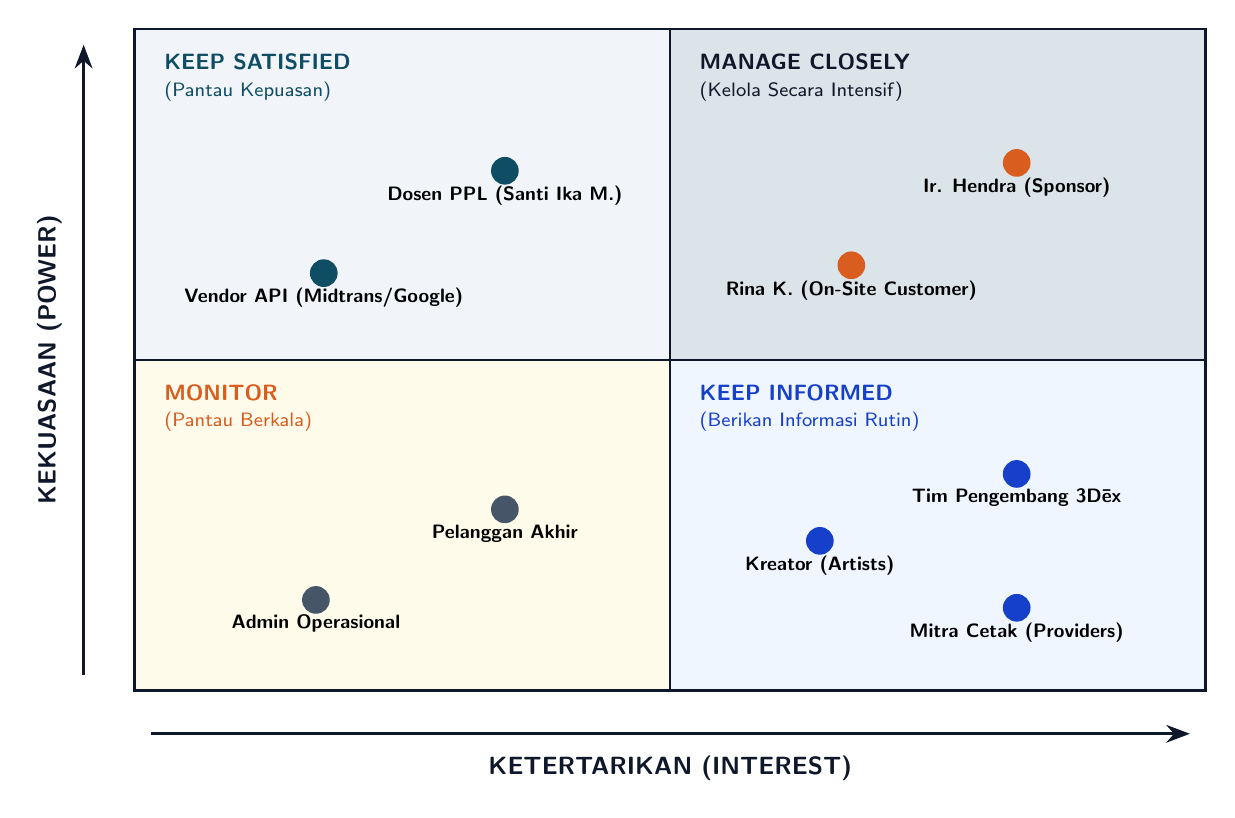
\begin{tikzpicture}[font=\sffamily\footnotesize]
    % Grid boxes (13.6cm x 8.4cm -> 6.8cm x 4.2cm per quadrant)
    \fill[lightslate] (0,4.2) rectangle (6.8,8.4);
    \fill[accentteal!15] (6.8,4.2) rectangle (13.6,8.4);
    \fill[softamber] (0,0) rectangle (6.8,4.2);
    \fill[softblue] (6.8,0) rectangle (13.6,4.2);

    \draw[brandnavy, line width=1pt] (0,0) rectangle (13.6,8.4);
    \draw[brandnavy, line width=0.9pt] (6.8,0) -- (6.8,8.4);
    \draw[brandnavy, line width=0.9pt] (0,4.2) -- (13.6,4.2);

    % Quadrant Titles (2-line compact titles, safely inside borders)
    \node[anchor=north west, align=left, font=\sffamily\footnotesize, text=accentteal] at (0.25, 8.2) {\textbf{KEEP SATISFIED}\\{\scriptsize (Pantau Kepuasan)}};
    \node[anchor=north west, align=left, font=\sffamily\footnotesize, text=brandnavy] at (7.05, 8.2) {\textbf{MANAGE CLOSELY}\\{\scriptsize (Kelola Secara Intensif)}};
    \node[anchor=north west, align=left, font=\sffamily\footnotesize, text=accentorange] at (0.25, 4.0) {\textbf{MONITOR}\\{\scriptsize (Pantau Berkala)}};
    \node[anchor=north west, align=left, font=\sffamily\footnotesize, text=brandblue] at (7.05, 4.0) {\textbf{KEEP INFORMED}\\{\scriptsize (Berikan Informasi Rutin)}};

    % Axes Labels
    \draw[-{Stealth[length=3mm]}, line width=1.1pt, brandnavy] (-0.65, 0.2) -- (-0.65, 8.2) node[midway, sloped, above=4pt, font=\sffamily\small\bfseries] {KEKUASAAN (POWER)};
    \draw[-{Stealth[length=3mm]}, line width=1.1pt, brandnavy] (0.2, -0.55) -- (13.4, -0.55) node[midway, below=4pt, font=\sffamily\small\bfseries] {KETERTARIKAN (INTEREST)};

    % Manage Closely (High Power, High Interest: x in [6.8..13.6], y in [4.2..8.4])
    \fill[accentorange] (11.2, 6.7) circle (5pt);
    \node[below=2pt, font=\sffamily\scriptsize\bfseries] at (11.2, 6.7) {Ir. Hendra (Sponsor)};

    \fill[accentorange] (9.1, 5.4) circle (5pt);
    \node[below=2pt, font=\sffamily\scriptsize\bfseries] at (9.1, 5.4) {Rina K. (On-Site Customer)};

    % Keep Satisfied (High Power, Low-Med Interest: x in [0..6.8], y in [4.2..8.4])
    \fill[accentteal] (4.7, 6.6) circle (5pt);
    \node[below=2pt, font=\sffamily\scriptsize\bfseries] at (4.7, 6.6) {Dosen PPL (Santi Ika M.)};

    \fill[accentteal] (2.4, 5.3) circle (5pt);
    \node[below=2pt, font=\sffamily\scriptsize\bfseries] at (2.4, 5.3) {Vendor API (Midtrans/Google)};

    % Keep Informed (Low-Med Power, High Interest: x in [6.8..13.6], y in [0..4.2])
    \fill[brandblue] (11.2, 2.75) circle (5pt);
    \node[below=2pt, font=\sffamily\scriptsize\bfseries] at (11.2, 2.75) {Tim Pengembang 3D\={e}x};

    \fill[brandblue] (8.7, 1.9) circle (5pt);
    \node[below=2pt, font=\sffamily\scriptsize\bfseries] at (8.7, 1.9) {Kreator (Artists)};

    \fill[brandblue] (11.2, 1.05) circle (5pt);
    \node[below=2pt, font=\sffamily\scriptsize\bfseries] at (11.2, 1.05) {Mitra Cetak (Providers)};

    % Monitor (Low Power, Low-Med Interest: x in [0..6.8], y in [0..4.2])
    \fill[mutedtext] (4.7, 2.3) circle (5pt);
    \node[below=2pt, font=\sffamily\scriptsize\bfseries] at (4.7, 2.3) {Pelanggan Akhir};

    \fill[mutedtext] (2.3, 1.15) circle (5pt);
    \node[below=2pt, font=\sffamily\scriptsize\bfseries] at (2.3, 1.15) {Admin Operasional};
\end{tikzpicture}
\caption{Pemetaan Stakeholder pada Power / Interest Grid}
\end{figure}

\begin{table}[H]
\centering
\caption{Ringkasan Frekuensi dan Kanal Komunikasi Pemangku Kepentingan}
\small
\begin{tabularx}{\textwidth}{| L{3.6cm} | L{3.0cm} | Y |}
\hline
\rowcolor{accentteal} \color{white}\textbf{Kuadran Strategis} & \color{white}\textbf{Frekuensi} & \color{white}\textbf{Kanal \& Artefak Komunikasi Utama} \\
\hline
Manage Closely & Mingguan / Per Fase & \textit{Planning Game}, demo rilis dua mingguan, persetujuan \textit{Change Request}, BAST. \\
\hline
Keep Satisfied & Per Milestone (M1 s.d. M5) & Pengumpulan draf Charter, laporan kemajuan proyek, pemantauan kuota API SLA. \\
\hline
Keep Informed & Harian / Pra-Rilis & \textit{Daily stand-up}, GitHub PR/CI log, undangan beta UAT Kreator \& Provider. \\
\hline
Monitor & Insidental / Pasca-Rilis & Umpan balik uji coba beta, tiket laporan penyalahgunaan, catatan audit sistem. \\
\hline
\end{tabularx}
\end{table}

\clearpage

% ==============================================================================
% LAMPIRAN B: RINGKASAN MILESTONE, SIKLUS HYBRID XP/PXP & USER STORIES
% ==============================================================================
\section{Ringkasan Milestone, Siklus Hybrid (XP/PXP), dan Daftar User Story}

\subsection{Pemilihan Siklus Hidup Proyek Hybrid}
Pengembangan 3D\={e}x menerapkan siklus hidup Hybrid:
\begin{enumerate}[leftmargin=1.5em, itemsep=2pt]
    \item \textit{Inisiasi dan Project Charter secara Prediktif:} Penetapan batasan lingkup, anggaran kontrak tetap Rp 148.500.000, tata kelola risiko, dan tenggat serah terima 106 hari dilakukan di awal secara formal.
    \item \textit{Eksekusi Pengembangan dengan Iterasi Agile Extreme Programming (XP) \& Personal Extreme Programming (PXP):} Karena tim beranggotakan 4 orang yang mengelola modul terpisah sekaligus berkolaborasi pada integrasi penuh, tim memadukan praktik inti XP (\textit{Planning Game}, \textit{Small Releases} per 2 hingga 3 minggu, \textit{Continuous Integration} harian, \textit{Pair Programming} pada WebGL/Midtrans/D\={e}xie, \textit{Collective Code Ownership}, dan \textit{On-Site Customer}) dengan siklus 7-langkah PXP (\textit{Requirements, Planning, Iteration Initialization, Design, Implementation, System Testing, Retrospective}) untuk pengembangan modul independen.
    \item \textit{Akselerasi 4GT/5GT:} Pemanfaatan Prisma ORM, Tailwind CSS, dan alat bantu AI berbatas kendali tinjauan manusia wajib untuk mempercepat pembuatan kode \textit{boilerplate} tanpa mengorbankan standar kualitas.
\end{enumerate}

\subsection{Bagan Gantt Jadwal Milestone (Minggu 1 s.d. 15 / 106 Hari)}

\begin{figure}[H]
\centering
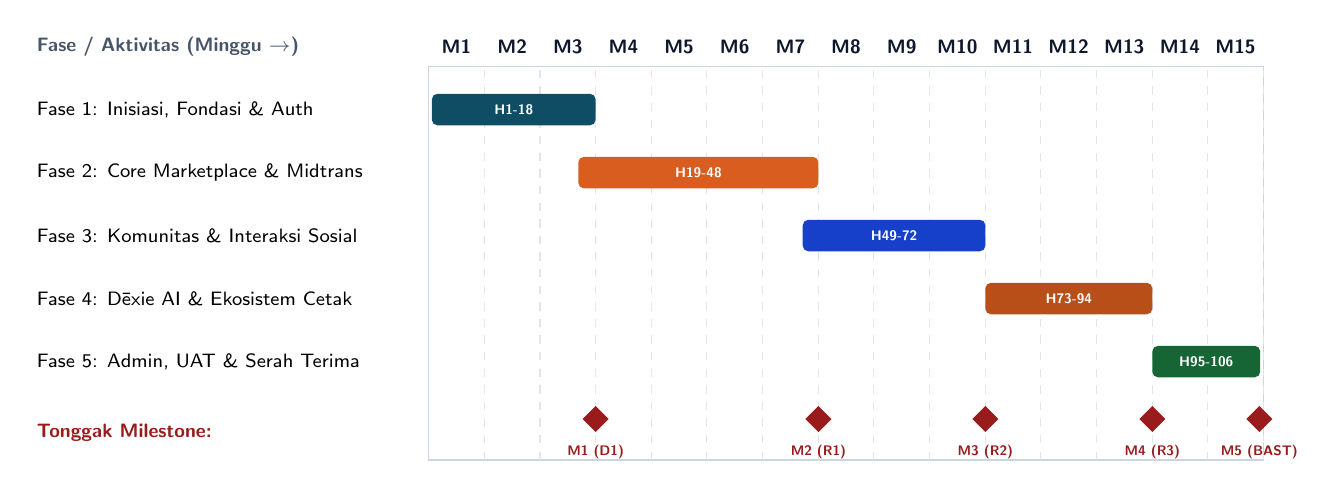
\begin{tikzpicture}[font=\sffamily\scriptsize]
    % Grid & Week headers
    \draw[bordergray] (5.10, 0.2) rectangle (15.70, 5.2);
    \foreach \w in {1,...,15} {
        \pgfmathsetmacro{\xpos}{5.10 + (\w - 0.5) * (10.60 / 15)}
        \node[font=\sffamily\scriptsize\bfseries, text=brandnavy] at (\xpos, 5.45) {M\w};
        \draw[bordergray!60, dashed] ({5.10 + \w * (10.60/15)}, 0.2) -- ({5.10 + \w * (10.60/15)}, 5.2);
    }
    \node[anchor=west, font=\sffamily\scriptsize\bfseries, text=mutedtext] at (0, 5.45) {Fase / Aktivitas (Minggu $\rightarrow$)};

    % Row labels & bars (15 weeks mapped to 10.60 width -> 1 week = 0.7067)
    % Row 1: Fase 1 (W1-W3)
    \node[anchor=west] at (0, 4.65) {Fase 1: Inisiasi, Fondasi \& Auth};
    \fill[accentteal, rounded corners=2pt] (5.14, 4.45) rectangle (7.22, 4.85);
    \node[white, font=\sffamily\tiny\bfseries] at (6.18, 4.65) {H1-18};

    % Row 2: Fase 2 (W3-W7)
    \node[anchor=west] at (0, 3.85) {Fase 2: Core Marketplace \& Midtrans};
    \fill[accentorange, rounded corners=2pt] (7.00, 3.65) rectangle (10.05, 4.05);
    \node[white, font=\sffamily\tiny\bfseries] at (8.525, 3.85) {H19-48};

    % Row 3: Fase 3 (W7-W10)
    \node[anchor=west] at (0, 3.05) {Fase 3: Komunitas \& Interaksi Sosial};
    \fill[brandblue, rounded corners=2pt] (9.85, 2.85) rectangle (12.17, 3.25);
    \node[white, font=\sffamily\tiny\bfseries] at (11.01, 3.05) {H49-72};

    % Row 4: Fase 4 (W11-W13)
    \node[anchor=west] at (0, 2.25) {Fase 4: D\={e}xie AI \& Ekosistem Cetak};
    \fill[accentorange!85!black, rounded corners=2pt] (12.17, 2.05) rectangle (14.29, 2.45);
    \node[white, font=\sffamily\tiny\bfseries] at (13.23, 2.25) {H73-94};

    % Row 5: Fase 5 (W14-W15)
    \node[anchor=west] at (0, 1.45) {Fase 5: Admin, UAT \& Serah Terima};
    \fill[accentgreen, rounded corners=2pt] (14.29, 1.25) rectangle (15.66, 1.65);
    \node[white, font=\sffamily\tiny\bfseries] at (14.975, 1.45) {H95-106};

    % Milestones diamonds at bottom
    \node[anchor=west, font=\sffamily\scriptsize\bfseries, text=accentred] at (0, 0.55) {Tonggak Milestone:};
    \foreach \x/\lbl in {7.22/M1 (D1), 10.05/M2 (R1), 12.17/M3 (R2), 14.29/M4 (R3), 15.65/M5 (BAST)} {
        \node[diamond, fill=accentred, inner sep=2.4pt] at (\x, 0.72) {};
        \node[below=1pt, font=\sffamily\tiny\bfseries, text=accentred] at (\x, 0.55) {\lbl};
    }
\end{tikzpicture}
\caption{Ringkasan Jadwal Milestone 15 Minggu (106 Hari Kalender) Selaras Iterasi XP}
\end{figure}

\subsection{Daftar Lengkap 26 User Story dan Alokasi Fase (Total: 106 Hari-Orang)}

{\footnotesize
\setlength{\tabcolsep}{4.2pt}
\begin{longtable}{| C{1.60cm} | C{1.40cm} | L{5.65cm} | L{4.00cm} | C{0.80cm} | C{1.05cm} |}
\caption{Daftar Lengkap User Story Platform 3D\={e}x} \\
\hline
\rowcolor{brandnavy} \color{white}\textbf{ID} & \color{white}\textbf{Aktor} & \color{white}\textbf{Saya ingin...} & \color{white}\textbf{Sehingga...} & \color{white}\textbf{Prio} & \color{white}\textbf{Est. (Hr)} \\
\hline
\endfirsthead
\hline
\rowcolor{brandnavy} \color{white}\textbf{ID} & \color{white}\textbf{Aktor} & \color{white}\textbf{Saya ingin...} & \color{white}\textbf{Sehingga...} & \color{white}\textbf{Prio} & \color{white}\textbf{Est. (Hr)} \\
\hline
\endhead
\hline
\endfoot
\texttt{US-GST-01} & Guest & Menjelajahi katalog publik dan berinteraksi dengan pemirsa 3D WebGL & Dapat menilai kualitas topologi aset sebelum mendaftar & 1 & 5 \\
\hline
\texttt{US-GST-02} & Guest & Mendaftar akun baru via lokal atau Google OAuth 2.0 & Dapat mengakses keranjang dan fitur terpersonalisasi & 1 & 4 \\
\hline
\texttt{US-CUS-01} & Customer & Mengelola profil, keamanan 2FA, dan visibilitas konten NSFW & Dapat mengamankan akun dan preferensi penjelajahan & 1 & 4 \\
\hline
\texttt{US-CUS-02} & Customer & Mencari model dengan filter teks maupun pencarian semantik AI & Dapat menemukan aset sesuai maksud pengguna secara cepat & 1 & 5 \\
\hline
\texttt{US-CUS-03} & Customer & Menyusun keranjang dan melakukan pembayaran via Midtrans Snap & Dapat membeli aset digital secara aman dengan metode lokal & 1 & 7 \\
\hline
\texttt{US-CUS-04} & Customer & Menerima tautan unduhan bertanda tangan pasca-pembayaran & Dapat segera mengunduh aset digital yang telah dibeli & 1 & 4 \\
\hline
\texttt{US-CUS-05} & Customer & Mengirimkan permintaan cetak 3D beserta spesifikasi material/skala & Model yang dibeli dapat diproduksi fisik oleh Provider & 1 & 6 \\
\hline
\texttt{US-CUS-06} & Customer & Melacak status pekerjaan cetak dan pengiriman secara \textit{real-time} & Mengetahui perkembangan pengiriman fisik secara pasti & 2 & 4 \\
\hline
\texttt{US-CUS-07} & Customer & Memberikan peringkat bintang dan ulasan pada aset yang dibeli & Berkontribusi terhadap sinyal kualitas layanan di platform & 2 & 4 \\
\hline
\texttt{US-CUS-08} & Customer & Mengikuti kreator dan berinteraksi di umpan sosial & Dapat membangun jejaring dan mengikuti karya terbaru & 3 & 5 \\
\hline
\texttt{US-CUS-09} & Customer & Menerima notifikasi aktivitas dan mengelompokkan model ke koleksi & Dapat mengelola minat dan aktivitas komunitas & 3 & 3 \\
\hline
\texttt{US-DEX-01} & Customer & Menerima rekomendasi personal dari D\={e}xie AI & Menemukan model relevan tanpa pencarian manual & 2 & 5 \\
\hline
\texttt{US-ART-01} & Artist & Mengunggah berkas 3D (\texttt{.glb/.gltf}) dengan lisensi ganda & Dapat memonetisasi karya digital (pribadi/komersial) & 1 & 7 \\
\hline
\texttt{US-ART-02} & Artist & Menetapkan model sebagai gratis atau berbayar & Dapat mengendalikan strategi komersial tiap aset & 1 & 4 \\
\hline
\texttt{US-ART-03} & Artist & Membuat unggahan portofolio dengan gambar render dan takarir & Memamerkan karya dan menarik trafik ke toko kreator & 2 & 5 \\
\hline
\texttt{US-ART-04} & Artist & Melihat analitik penjualan dan mengajukan pencairan dana & Dapat memantau kinerja pendapatan dan penarikan saldo & 2 & 3 \\
\hline
\texttt{US-PRV-01} & Provider & Mengelola pesanan cetak masuk serta menerima/menolak pekerjaan & Dapat mengontrol antrean produksi bengkel cetak & 1 & 4 \\
\hline
\texttt{US-PRV-02} & Provider & Mengunduh berkas sumber \texttt{.glb} pelanggan untuk produksi & Memiliki berkas 3D akurat yang siap dicetak & 1 & 4 \\
\hline
\texttt{US-PRV-03} & Provider & Mengisi nomor resi pengiriman dan foto bukti kerja & Pelanggan memiliki bukti terverifikasi atas proses kirim & 1 & 4 \\
\hline
\texttt{US-ADM-01} & Admin & Memoderasi pengajuan peran Artist dan Provider & Memastikan hanya mitra terverifikasi yang mendapat akses & 1 & 3 \\
\hline
\texttt{US-ADM-02} & Admin & Meninjau dan menyetujui/menolak model 3D yang baru diunggah & Menjaga standar kualitas konten sebelum tayang publik & 1 & 3 \\
\hline
\texttt{US-ADM-03} & Admin & Menangani laporan penyalahgunaan dan sengketa komunitas & Menjaga integritas dan keamanan ekosistem platform & 1 & 4 \\
\hline
\texttt{US-ADM-04} & Admin & Memantau statistik transaksi dan kesehatan platform terpadu & Mengawasi kinerja operasional platform secara menyeluruh & 2 & 2 \\
\hline
\texttt{US-ADM-05} & Admin & Meninjau catatan \textit{audit log} seluruh tindakan administratif & Menjamin transparansi dan akuntabilitas moderasi & 2 & 2 \\
\hline
\texttt{US-ADM-06} & Admin & Memberi peringatan, menangguhkan, atau memblokir akun nakal & Menegakkan kepatuhan aturan komunitas & 1 & 3 \\
\hline
\texttt{US-SYS-01} & Tim Sistem & Melaksanakan pengujian regresi penuh dan audit performa sistem & Memastikan platform stabil dan siap produksi komersial & 2 & 2 \\
\hline
\rowcolor{softblue} \multicolumn{5}{|r|}{\textbf{Total Estimasi Usaha Pengembangan (26 User Story across 5 Fase)}} & \textbf{106} \\
\hline
\end{longtable}
}
\normalsize

\clearpage

% ==============================================================================
% LAMPIRAN C: ESTIMASI ANGGARAN, PERHITUNGAN PERT & KOMPOSISI BIAYA
% ==============================================================================
\section{Estimasi Anggaran, Perhitungan PERT, dan Komposisi Biaya}

\subsection{Dasar Perhitungan: Metode Three-Point (PERT) dan Parametric}
Untuk menghasilkan anggaran yang objektif sebelum kode pertama ditulis, tim rekayasa menggunakan dua teknik estimasi standar PMBOK\textsuperscript{\textregistered} Guide Edisi 6:
\begin{enumerate}[leftmargin=1.5em, itemsep=2pt]
    \item \textit{Three-Point Estimation (PERT):} Menghitung perkiraan usaha hari-orang (\textit{person-days}) per fase berdasarkan nilai Optimis ($O$), Paling Mungkin ($M$), dan Pesimis ($P$) menggunakan rumus rata-rata berbobot:
    \[
        E = \frac{O + 4M + P}{6}, \qquad \sigma = \frac{P - O}{6}
    \]
    \item \textit{Parametric Estimation:} Mengalikan total ekspektasi usaha pengembangan ($E_{\text{total}} = 106{,}0\text{ hari-orang}$) dengan tarif tenaga rekayasa komersial PT Schryzon Digital Nusantara sebesar Rp 1.000.000 per hari-orang, kemudian menjumlahkannya dengan komponen infrastruktur dan cadangan risiko 10\%.
\end{enumerate}

\begin{table}[H]
\centering
\caption{Perhitungan Usaha dan Biaya Pengembangan Menggunakan Metode PERT}
\begin{tabularx}{\textwidth}{| Y | C{0.85cm} | C{0.85cm} | C{0.85cm} | C{1.55cm} | C{1.05cm} | R{3.2cm} |}
\hline
\rowcolor{brandnavy} \color{white}\textbf{Fase / Modul Pengembangan} & \color{white}\textbf{$O$} & \color{white}\textbf{$M$} & \color{white}\textbf{$P$} & \color{white}\textbf{$E$ (Hr-Org)} & \color{white}\textbf{$\sigma$} & \color{white}\textbf{Biaya (Parametric)} \\
\hline
Fase 1: Fondasi, DB \& Auth & 8 & 11 & 14 & 11,0 & 1,00 & Rp 11.000.000 \\
\hline
Fase 2: Core Marketplace \& Midtrans & 28 & 35 & 42 & 35,0 & 2,33 & Rp 35.000.000 \\
\hline
Fase 3: Komunitas \& Fitur Sosial & 16 & 21 & 26 & 21,0 & 1,67 & Rp 21.000.000 \\
\hline
Fase 4: D\={e}xie AI \& Ekosistem Cetak & 20 & 27 & 34 & 27,0 & 2,33 & Rp 27.000.000 \\
\hline
Fase 5: Admin, QA Regresi \& Rilis & 9 & 12 & 15 & 12,0 & 1,00 & Rp 12.000.000 \\
\hline
\rowcolor{softblue} \textbf{Total Usaha Rekayasa (PERT)} & \textbf{81} & \textbf{106} & \textbf{131} & \textbf{106,0} & \textbf{8,33} & \textbf{Rp 106.000.000} \\
\hline
\end{tabularx}
\end{table}

\subsection{Rincian Anggaran Keseluruhan dan Komposisi Biaya}

\begin{table}[H]
\centering
\caption{Rincian Komponen Anggaran Proyek 3D\={e}x (Disetujui Sponsor)}
\begin{tabularx}{\textwidth}{| L{5.2cm} | Y | R{3.2cm} | C{1.5cm} |}
\hline
\rowcolor{accentteal} \color{white}\textbf{Komponen Biaya} & \color{white}\textbf{Keterangan Rincian} & \color{white}\textbf{Nilai (IDR)} & \color{white}\textbf{Porsi} \\
\hline
1. Tenaga Pengembang Perangkat Lunak & $106\text{ hari-orang} \times \text{Rp }1.000.000$ (4 Personil) & Rp 106.000.000 & 71,38\% \\
\hline
2. Infrastruktur Cloud, VPS, MinIO S3 \& API & Hosting 12 Bulan (FE/\allowbreak BE/\allowbreak PGVector/\allowbreak MinIO), SSL, Kuota Gemini \& Midtrans & Rp 16.500.000 & 11,11\% \\
\hline
3. Sistem Desain UI/UX, WebGL \& QA & Aset Desain Tema Gelap, Pengujian Regresi \& Audit Performa & Rp 7.500.000 & 5,05\% \\
\hline
4. Dokumentasi, Pelatihan \& Workshop UAT & Manual Pengguna/Admin, BAST, Sesi Pelatihan Staf Krea3D Corp & Rp 5.000.000 & 3,37\% \\
\hline
\rowcolor{lightslate} \textbf{Subtotal Biaya Dasar} & \textbf{Total Pengeluaran Terencana} & \textbf{Rp 135.000.000} & \textbf{90,91\%} \\
\hline
5. Cadangan Risiko (\textit{Risk Contingency}) & 10\% dari Subtotal untuk Mitigasi Risiko R-01 s.d. R-06 & Rp 13.500.000 & 9,09\% \\
\hline
\rowcolor{softblue} \textbf{TOTAL ANGGARAN DISETUJUI} & \textbf{Kontrak Tetap PT Kreasi Tiga Dimensi Indonesia} & \textbf{Rp 148.500.000} & \textbf{100,00\%} \\
\hline
\end{tabularx}
\end{table}

\begin{figure}[H]
\centering
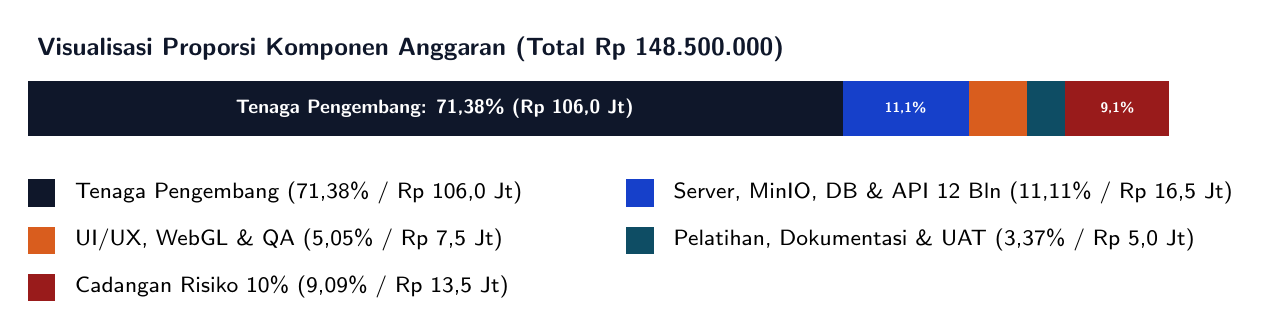
\begin{tikzpicture}[font=\sffamily\footnotesize]
    \node[anchor=west, font=\sffamily\small\bfseries, text=brandnavy] at (0, 3.3) {Visualisasi Proporsi Komponen Anggaran (Total Rp 148.500.000)};

    % Horizontal stacked bar (width 14.5 cm)
    \fill[brandnavy] (0, 2.2) rectangle (10.35, 2.9);       % 71.38% -> 10.35
    \fill[brandblue] (10.35, 2.2) rectangle (11.96, 2.9);   % 11.11% -> 1.61
    \fill[accentorange] (11.96, 2.2) rectangle (12.69, 2.9);% 5.05% -> 0.73
    \fill[accentteal] (12.69, 2.2) rectangle (13.18, 2.9);  % 3.37% -> 0.49
    \fill[accentred] (13.18, 2.2) rectangle (14.50, 2.9);   % 9.09% -> 1.32

    \node[white, font=\sffamily\scriptsize\bfseries] at (5.17, 2.55) {Tenaga Pengembang: 71,38\% (Rp 106,0 Jt)};
    \node[white, font=\sffamily\tiny\bfseries] at (11.15, 2.55) {11,1\%};
    \node[white, font=\sffamily\tiny\bfseries] at (13.84, 2.55) {9,1\%};

    % Legend (2 spacious columns inside 14.5cm width)
    \fill[brandnavy] (0, 1.3) rectangle (0.35, 1.65);
    \node[anchor=west] at (0.48, 1.48) {Tenaga Pengembang (71,38\% / Rp 106,0 Jt)};

    \fill[brandblue] (7.6, 1.3) rectangle (7.95, 1.65);
    \node[anchor=west] at (8.08, 1.48) {Server, MinIO, DB \& API 12 Bln (11,11\% / Rp 16,5 Jt)};

    \fill[accentorange] (0, 0.7) rectangle (0.35, 1.05);
    \node[anchor=west] at (0.48, 0.88) {UI/UX, WebGL \& QA (5,05\% / Rp 7,5 Jt)};

    \fill[accentteal] (7.6, 0.7) rectangle (7.95, 1.05);
    \node[anchor=west] at (8.08, 0.88) {Pelatihan, Dokumentasi \& UAT (3,37\% / Rp 5,0 Jt)};

    \fill[accentred] (0, 0.1) rectangle (0.35, 0.45);
    \node[anchor=west] at (0.48, 0.28) {Cadangan Risiko 10\% (9,09\% / Rp 13,5 Jt)};
\end{tikzpicture}
\caption{Komposisi Anggaran Proyek Komersial 3D\={e}x}
\end{figure}

\clearpage

% ==============================================================================
% LAMPIRAN D: DAFTAR RESOURCE & MATRIKS RACI
% ==============================================================================
\section{Daftar Resource (Tim, Peran XP \& Sarana) serta Matriks RACI}

\subsection{Tim Proyek dan Pemetaan Peran Extreme Programming (XP)}

\begin{table}[H]
\centering
\caption{Daftar Personil Tim Inti, Peran XP, dan Tanggung Jawab}
\begin{tabularx}{\textwidth}{| L{4.2cm} | C{2.3cm} | L{3.2cm} | Y |}
\hline
\rowcolor{brandnavy} \color{white}\textbf{Nama Personil} & \color{white}\textbf{NIM / ID} & \color{white}\textbf{Peran XP} & \color{white}\textbf{Domain Kepemilikan Utama} \\
\hline
I Nyoman Widiyasa Jayananda (\texttt{Schryzon}) & \texttt{F1D02410053} & PM / Tracker \& Programmer & Arsitektur Backend Express.js, Prisma PostgreSQL/\texttt{pgvector}, MinIO S3, D\={e}xie AI, CI/CD, Docker \& SysAdmin. \\
\hline
I Kadek Mahesa Permana Putra (\texttt{Vuxyn}) & \texttt{F1D02410052} & Programmer \& Tester (QA Lead) & Frontend Next.js App Router, \textit{Design System} Tema Gelap, Pemirsa WebGL Three.js, Pengujian Regresi \& Performa. \\
\hline
Thoriq Abdillah Falian Kusuma (\texttt{ganijack}) & \texttt{F1D02410098} & Programmer & Integrasi Frontend-Backend, Alur Autentikasi Google OAuth 2.0, Midtrans Snap, Modul Cetak 3D \& Notifikasi. \\
\hline
Ni Putu Ayu Dian Sulastri & \texttt{F1D02510021} & Customer Liaison / Analyst & Analisis Kebutuhan Bisnis, Penyusunan Dokumentasi Charter/UML, Koordinasi UAT \& Pelatihan Klien. \\
\hline
Rina Kusumawardhani (Krea3D Corp) & \texttt{KREA3D-PO} & On-Site Customer & Penentuan prioritas \textit{User Story} pada \textit{Planning Game}, verifikasi demo rilis, dan persetujuan UAT. \\
\hline
\end{tabularx}
\end{table}

\subsection{Daftar Sarana Perangkat Keras, Perangkat Lunak, dan Infrastruktur}
\begin{itemize}[leftmargin=1.5em, itemsep=2pt]
    \item \textit{Perangkat Keras Tim Pengembang:} 4 unit Workstation/Laptop Rekayasa (Prosesor setara Ryzen 6800H / Core i7, RAM 16 hingga 32 GB, GPU berkemampuan WebGL 2.0) untuk pengembangan lokal dan rendering uji 3D.
    \item \textit{Perangkat Lunak \& Alat Kolaborasi:} Visual Studio Code / Antigravity IDE, Git \& GitHub Private Repository dengan GitHub Actions CI/CD, Docker \& Docker Compose, Node.js 20 LTS, PostgreSQL 16 + \texttt{pgvector}, MinIO Server, XeLaTeX \& PlantUML untuk dokumentasi arsitektur.
    \item \textit{Infrastruktur Uji \& Produksi (4 Node):} Server Cloud / VPS Produksi (Node Frontend, Node Backend Modular Monolith, Node Database PostgreSQL 16, Node Penyimpanan Objek MinIO S3), serta akun Sandbox \& Produksi Midtrans Snap dan Google Cloud Gemini API.
\end{itemize}

\subsection{Matriks Tanggung Jawab (RACI Matrix)}
Keterangan peran RACI: \textbf{R} = \textit{Responsible} (Pelaksana), \textbf{A} = \textit{Accountable} (Pemegang Akuntabilitas Tunggal per Aktivitas), \textbf{C} = \textit{Consulted} (Dimintai Masukan), \textbf{I} = \textit{Informed} (Diinformasikan).

\begin{table}[H]
\centering
\caption{Matriks RACI untuk 14 Domain Aktivitas Utama Proyek 3D\={e}x}
\footnotesize
\begin{tabularx}{\textwidth}{| Y | C{1.6cm} | C{1.6cm} | C{1.6cm} | C{1.6cm} | C{1.6cm} |}
\hline
\rowcolor{accentteal} \color{white}\textbf{Aktivitas / Domain Proyek} & \color{white}\textbf{Jay (PM/BE)} & \color{white}\textbf{Mahesa (FE/QA)} & \color{white}\textbf{Thoriq (Integ.)} & \color{white}\textbf{Dian (BA/Doc)} & \color{white}\textbf{Rina (Cust.)} \\
\hline
1. Penyusunan Project Charter v1.0 & \textbf{A/R} & C & C & R & C \\
\hline
2. Penulisan \& Prioritas User Story & R & C & C & R & \textbf{A} \\
\hline
3. Desain Skema DB \& Migrasi Prisma & \textbf{A/R} & I & C & C & I \\
\hline
4. Implementasi REST API Modular Monolith & \textbf{A/R} & C & R & I & I \\
\hline
5. Desain Sistem UI/UX \& WebGL Viewer & C & \textbf{A/R} & C & I & C \\
\hline
6. Autentikasi JWT \& Google OAuth 2.0 & C & I & \textbf{A/R} & I & I \\
\hline
7. Integrasi Pembayaran Midtrans Snap & R & I & \textbf{A/R} & I & C \\
\hline
8. Penyimpanan Objek MinIO S3 (\texttt{.glb}) & \textbf{A/R} & I & C & I & I \\
\hline
9. Mesin Rekomendasi D\={e}xie AI (\texttt{pgvector}) & \textbf{A/R} & C & I & I & C \\
\hline
10. Alur Pesanan Cetak 3D \& Dasbor Provider & C & C & \textbf{A/R} & C & C \\
\hline
11. Fitur Komunitas, Ulasan \& Notifikasi & R & C & \textbf{A/R} & I & I \\
\hline
12. Dasbor Admin, Moderasi \& Audit Log & \textbf{A/R} & C & R & C & I \\
\hline
13. Pengujian Regresi, Performa \& UAT & C & \textbf{A/R} & C & R & R \\
\hline
14. Demo Rilis, Pelatihan \& Serah Terima & R & R & R & R & \textbf{A} \\
\hline
\end{tabularx}
\end{table}

\clearpage

% ==============================================================================
% LAMPIRAN E: CHECKLIST VERIFIKASI CHARTER & DIAGRAM USE CASE
% ==============================================================================
\section{Checklist Verifikasi Project Charter dan Diagram Use Case}

\subsection{Checklist Kesiapan Pengumpulan Charter (Standar Kuliah PPL UNRAM)}

\begin{table}[H]
\centering
\caption{Checklist Evaluasi Mandiri Project Charter v1.0 Sebelum Pengumpulan}
\begin{tabularx}{\textwidth}{| C{0.9cm} | Y | C{2.7cm} | C{2.2cm} |}
\hline
\rowcolor{brandnavy} \color{white}\textbf{No} & \color{white}\textbf{Kriteria Verifikasi Kelengkapan Project Charter} & \color{white}\textbf{Lokasi Bagian} & \color{white}\textbf{Status} \\
\hline
1 & Masalah bisnis klien tertulis jelas dan terukur, bukan sekadar daftar solusi teknis & Bagian 1 & \badge{accentgreen}{TERPENUHI} \\
\hline
2 & Tersedia tujuan terukur (SMART) beserta kriteria sukses proyek yang eksplisit & Bagian 2 & \badge{accentgreen}{TERPENUHI} \\
\hline
3 & Lingkup proyek memuat daftar ``Dalam Lingkup'' (\textit{In Scope}) dan ``Di Luar Lingkup'' (\textit{Out of Scope}) & Bagian 4.2 & \badge{accentgreen}{TERPENUHI} \\
\hline
4 & Deliverable utama (D1 s.d. D5) disusun jelas selaras per rilis iteratif & Bagian 4.3 & \badge{accentgreen}{TERPENUHI} \\
\hline
5 & Ringkasan jadwal milestone bertanggal lengkap dan selaras siklus XP/PXP & Bagian 6 \& Lampiran B & \badge{accentgreen}{TERPENUHI} \\
\hline
6 & Estimasi anggaran dilengkapi dasar perhitungan PERT/Parametric dan cadangan risiko 10\% & Bagian 7 \& Lampiran C & \badge{accentgreen}{TERPENUHI} \\
\hline
7 & Tersedia Stakeholder Register (Proses 13.1) dan pemetaan Power/Interest Grid & Lampiran A & \badge{accentgreen}{TERPENUHI} \\
\hline
8 & Peran tim XP, daftar sarana, dan Matriks RACI mematuhi aturan satu \textit{Accountable} per aktivitas & Lampiran D & \badge{accentgreen}{TERPENUHI} \\
\hline
9 & Risiko utama, asumsi, dan kendala tercatat dalam \textit{Risk Register} dan \textit{Assumption Log} & Bagian 5 & \badge{accentgreen}{TERPENUHI} \\
\hline
10 & Nama Sponsor, Project Manager, dan kolom tanda tangan pengesahan tersedia lengkap & Surat \& Bagian 12 & \badge{accentgreen}{TERPENUHI} \\
\hline
\end{tabularx}
\end{table}

\clearpage
\subsection{Diagram Use Case Ekosistem Platform 3D\={e}x}
Diagram di bawah ini mendokumentasikan batas interaksi seluruh aktor manusia dan aktor eksternal sistem (\textit{Guest, Customer, Artist, Provider, Admin, D\={e}xie AI, Midtrans, Delivery Service, Time}) yang dicakup dalam ruang lingkup Project Charter ini.

\begin{figure}[H]
    \centering
    \includegraphics[width=\textwidth]{c:/Users/nyoma/Downloads/3Dex/docs/diagrams/final_ucd_exported.png}
    \caption{Diagram Use Case Terpadu Platform Komersial 3D\={e}x}
\end{figure}

\end{document}
